\documentclass{beamer} %[12pt]
\usepackage{xcolor}
%\usetheme{boadilla}
%\usetheme{malmoe}
%\usetheme{copenhagen}
%\usecolortheme{rose}
\usecolortheme{beaver}
\usepackage{pgf, graphics}
\usepackage{graphicx}
%\usepackage[left=3cm,top=3cm,right=3cm,nohead,nofoot]{geometry}
\usepackage{hyperref}
\usepackage{setspace}
\usepackage[square]{natbib}
\usepackage{amsmath}
\usepackage{amssymb}
\usepackage{verbatim}
\usepackage{color}
\usepackage{fancyvrb}
\usepackage{bbm}

\begin{filecontents}{ref.bib}
\end{filecontents}

%\usetheme{EastLansing}
%\usepackage{natbib}
\bibliographystyle{apalike}
% make bibliography entries smaller
%\renewcommand\bibfont{\scriptsize}
% If you have more than one page of references, you want to tell beamer
% to put the continuation section label from the second slide onwards
\setbeamertemplate{frametitle continuation}[from second]
% Now get rid of all the colours
\setbeamercolor*{bibliography entry title}{fg=black}
\setbeamercolor*{bibliography entry author}{fg=black}
\setbeamercolor*{bibliography entry location}{fg=black}
\setbeamercolor*{bibliography entry note}{fg=black}
% and kill the abominable icon
\setbeamertemplate{bibliography item}{}


\newcommand{\hl}[1]{\colorbox{yellow}{#1}}
\newcommand{\hlblue}[1]{\colorbox{green}{#1}}
\newcommand{\hlblu}[1]{\colorbox{cyan}{#1}}
\newcommand{\hlred}[1]{\colorbox{cyan}{#1}}
\newcommand{\hlre}[1]{\colorbox{pink}{#1}}
\newcommand{\hlgreen}[1]{\colorbox{pink}{#1}}
\newcommand{\hlgree}[1]{\colorbox{green}{#1}}



\DeclareMathOperator*{\argmax}{\arg\!\max}

\DeclareMathOperator*{\argmin}{\arg\!\min}


\newcommand{\specialcell}[2][c]{%
  \begin{tabular}[#1]{@{}c@{}}#2\end{tabular}}



%\setbeamersize{text margin left=.5cm,text margin right=.5cm}
\newenvironment{changemargin}[2]{%
  \begin{list}{}{%
    \setlength{\topsep}{0pt}%
    \setlength{\leftmargin}{#1}%
    \setlength{\rightmargin}{#2}%
    \setlength{\listparindent}{\parindent}%
    \setlength{\itemindent}{\parindent}%
    \setlength{\parsep}{\parskip}%
  }%
  \item[]}{\end{list}}
\setbeamertemplate{navigation symbols}{}%remove navigation symbols
\usepackage{color}
\newcommand{\hilight}[1]{\colorbox{yellow}{#1}}
\setbeamertemplate{footline}[page number]

\begin{document}


\title[dedup]{Today:  Marginal and Conditional Distributions \\ 2-D Caterogical Data \\ Contingency Tables and Mosaic Plots \\ Friday:  2-D Categorical}


\author[Samuel L. Ventura]{\\
  \large{Sam Ventura\\36-315}}
\institute[CMU Statistics]{Department of Statistics\\Carnegie Mellon University}
\date{\today}


\begin{frame}
	\maketitle
	
\end{frame}




\begin{frame}\frametitle{Quarterbacks with Over 2000 Yards, 2010 -- 2013}
	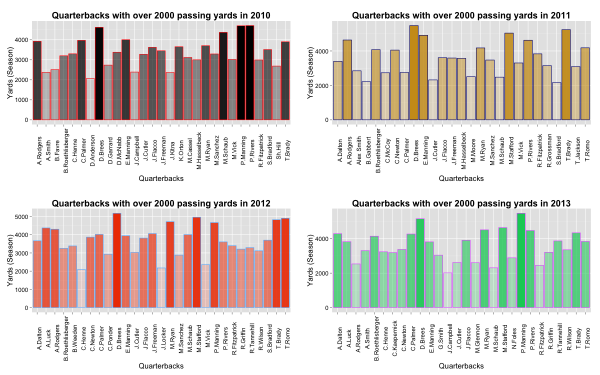
\includegraphics[width=\linewidth]{qbs.png}
\end{frame}




\begin{frame}\frametitle{2-D Categorical: Stacked and Side-by-Side Bar Charts}
	\small
	
	\textbf{2-D Bar Charts}:  %(more in lab on Friday)
	
	\vskip 5 cm
	
	\textbf{What does a 2-D bar chart show?}:  %Several conditional distributions\\
	
	%Conditional distribution of variable 2 given each category of variable 1
	
	
	\vskip 10 cm
	
\end{frame}





\begin{frame}\frametitle{Contingency Tables}
	\small
	
	\textbf{Contingency Tables Give Us}:  %Give us info about sample size\\
	
	\vskip 3 cm
	
	\textbf{Two Categorical Variables}:  %Give us info about sample size\\
	
	\vskip 1 cm
	
	\textbf{What Are We Interested In?}  %Give us info about sample size\\
	
	
	
	
	
	\vskip 10 cm
	
\end{frame}


\begin{frame}\frametitle{Contingency Tables and Marginal/Conditional Distributions}
	\small
	
	
	
\end{frame}



\begin{frame}\frametitle{Recall:  Independence Rules from Probability}
	\small
	
	\vskip 6 cm
	
	Can input contingency tables into chi-square tests for independence
	
	\vskip 0.5 cm
	
	E.g. \texttt{chisq.test(table(var1, var2))}
	
	\vskip 0.5 cm
	
	More on this in Lab 04
	
\end{frame}


\begin{frame}\frametitle{Pearson Residuals}
	\small
	
	\textbf{Pearson Residuals:}  Scaled difference between observed/expected%Give us info about sample size\\
	
	%But we could also get this by just including the sample size in the title of the chart
	
	\vskip 10 cm
	
\end{frame}



\begin{frame}\frametitle{Mosaic Plots}
	\small
	
	\textbf{Mosaic Plots}:  Area plot for two categorical variables%(more in lab on Friday)
	
	\vskip 6.6 cm
	
	\textbf{Can color the boxes by their differences from what was expected}  %Several conditional distributions\\
	
	\vskip 0.25 cm
	%Conditional distribution of variable 2 given each category of variable 1
	
	\textbf{Friday}:  Mosaic Plots in R%Several conditional distributions\\
	
	\vskip 10 cm
	
\end{frame}



\end{document}
